\chapter{Resimulaciones de Vacios Cosmol\'ogicos} % Main chapter title

\label{Voids} %



\section{Simulaci\'on Base}

Se realiz\'o una simulaci\'on \textit{base} de solo materia oscura en un \textit{box} cosmologico de 500 Mpc de lado con $512^{3}$ particulas. Para esto se utiliz\'o el c\'odigo \texttt{\textbf{MUSIC}} \citep{MUSIC} para la generaci\'on de condiciones iniciales (a z=50) mientras que la integraci\'on se llevo al cabo con el c\'odigo \texttt{\textbf{GIZMO}} \citep{GIZMO2015}. 

Sobre esta simulaci\'on se identificaron los halos de materia oscura utilizando el identificador de halos \texttt{\textbf{ROCKSTAR}} \citep{Rockstar}. 

La figura \ref{Base2snap} presenta dos \textit{snapshots} de la misma, uno a z=4 y otro a z=0. Podemos observar como la estructura evoluciona claramente a medida que pasa el tiempo. La simulaci\'on a z=4 presenta un universo mucho mas homog\'eneo que a z=0. Las regiones donde se vislumbra alguna sobre densidad o subdensidad en la primera, son muy amplificadas a z=0 contituyendo grandes vac\'ios o filamentos o nodos de mucha densidad. 


\begin{figure}
    \centering
    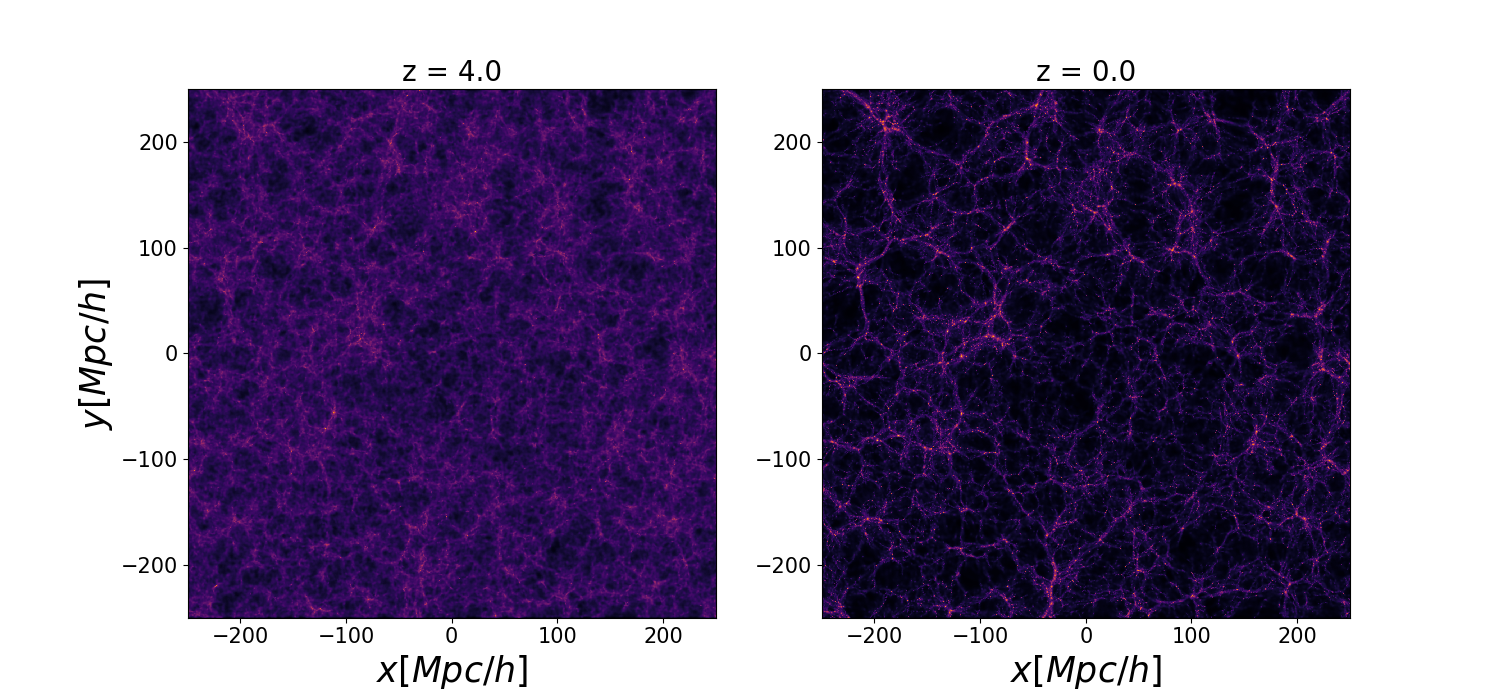
\includegraphics[width=15cm]{Figures/Base_2snap.png}
    \caption{Caption}
    \label{Base2snap}
\end{figure}{}

Tal como se menciono en la secci\'on \textbf{ALGUNA} la zonas de mas alta densidad atraen la materia por medio de su intenso potencial gravitacional. Con motivo de ilustrar este comportamiento se identifico una regi\'on de alta densidad y se calculo el campo de velocidad de el entorno. Esto se muestra en la figura \ref{Streamlines} donde podemos ver como las l\'ineas de campo de velocidad se dirigen hacia las zonas mas oscuras que corresponden a regiones de alta densidad. En la escala de colores de las l\'ineas se representa la intensidad de la velocidad. Se aprecia entonces que el campo alcanza su mayor intensidad en las proximidades de las zonas densas, siendo menores en los centros subdensos. 

\begin{figure}
    \centering
    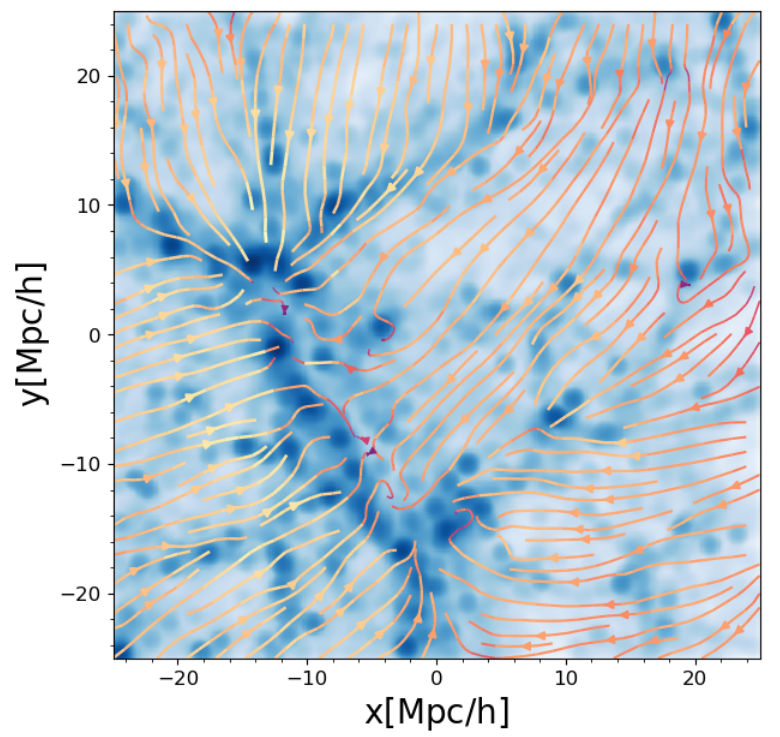
\includegraphics[width=13cm]{Figures/Streamlines.png}
    \caption{Caption}
    \label{Streamlines}
\end{figure}{}

\section{Identificaci\'on de Vac\'ios}

Con el algoritmo descripto en la secci\'on se identificaron los voids utilizados sobre la simulaci\'on \textit{base} utilizando el cat\'alogo de halos con un corte en 20 particulas. Los voids identificados entonces corresponden a los trazados por halos de $1.4$ $10^{12}M_{\odot}$. Sobre este cat\'alogo se identificaron 1384 voids. 
La figura \ref{VoidsIdentificados} es un corte transversal de la simulaci\'on donde las esferas marcan algunos de los voids identificados en la simulaci\'on. 

\begin{figure}
    \centering
    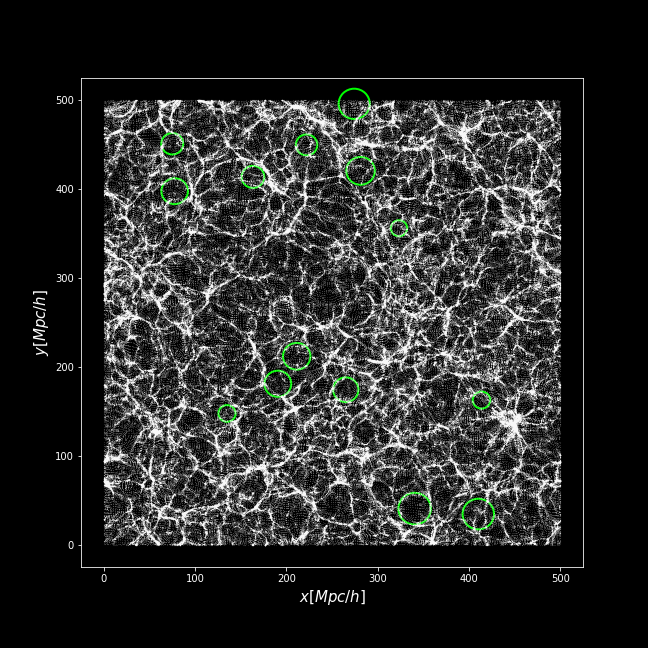
\includegraphics[width=12cm]{Figures/voids_r2.png}
    \caption{Caption}
    \label{VoidsIdentificados}
    
\end{figure}{}

Con el cat\'alogo de voids construido se contruyeron los perfiles de densidad integrada que pueden verse en la figure \ref{PerfilesVoids}. Cuando se observan los perfiles $\Delta$ los voids tienen dos tipos de comportamiento. Aquellos que alcanzan una $\Delta$ superior a la media del universo ($\Delta=0$) para luego decrecer hasta estabilizarse, y aquellos que crecen en $\Delta$ lentamente. Los primeros son los denominados voids \textbf{Tipo S} y los segundos los denominados \textbf{Tipo R}. Los tipo S presentan paredes muy sobredensas que se encuentran en proceso de colapso, esto produce que t\'ipicamente sean mas chicos que los tipo R \citep{Ceccarelli2013}.
\begin{figure}
    \centering
    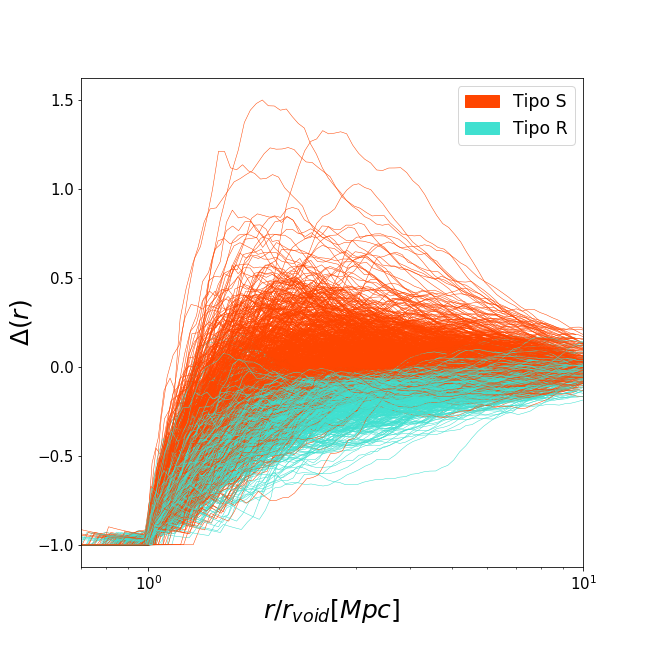
\includegraphics[width=12cm]{Figures/voids_sep.png}
    \caption{Caption}
    \label{PerfilesVoids}
\end{figure}{}

De la muestra de $\sim$ 1300 voids se seleccionaron 2, uno tipo S y uno R. Los perfiles de los voids seleccionados se presentan en la figura \ref{perfileshalos}. 

\begin{figure}
    \centering
    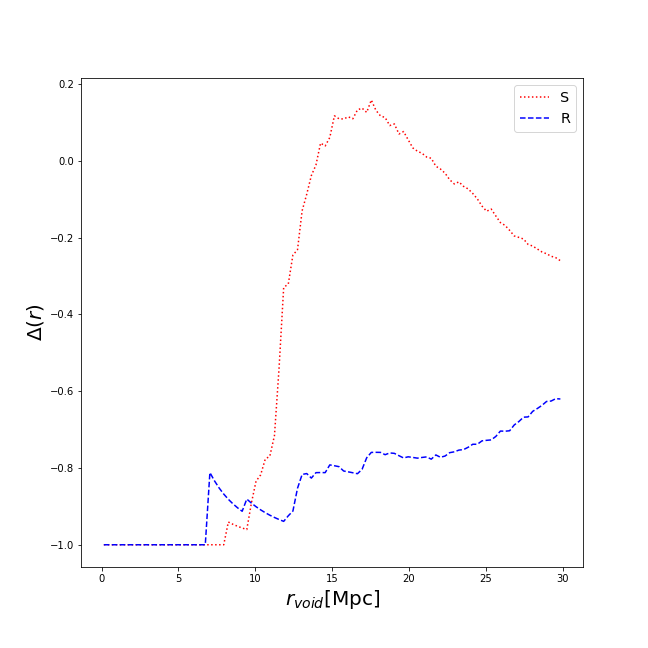
\includegraphics[width=\linewidth]{Figures/perfiles_halos.png}
    \caption{Caption}
    \label{perfileshalos}
\end{figure}{}

\section{Voids Resimulados}

Sobre el cat\'alogo de voids construidos se resimularon 2 vac\'ios, agregando particulsa de gas y recetas de \textit{feedback} y formaci\'on estelar siguiendo el modelo de \citet{Springel2003}. Un void tipo S y otro tipo R. Estos fueron seleccionados de modo que sean \textit{muy S y R} para de esta manera sean lo mas representativos posibles de la poblaci\'on general de cada tipo. Tanto la simulaci\'on \textit{base} como las resimulaciones fueron realizadas con el c\'odigo p\'ublico \texttt{\textbf{GIZMO}} \citep{GIZMO2015} y las condiciones iniciales iniciales se generan con el c\'odigo \texttt{\textbf{MUSIC}} \citep{MUSIC}. En la tabla \ref{Simulaciones0} del ap\'endice se presentan los datos de las simulaciones y resimulaciones utilizadas para este trabajo. 

En la figura \ref{Resi} se compara la regi\'on original de la simulaci\'on \textit{base} con su resimulaci\'on. Solo estamos representando particulas de materia oscura. Ambas son un corte transversal de 4 Mpc. Se observa que la estructura general es la misma en ambas simulaciones, pero obteniendose mayor resoluci\'on en el caso de la resimulaci\'on. 

\begin{figure}
    \centering
    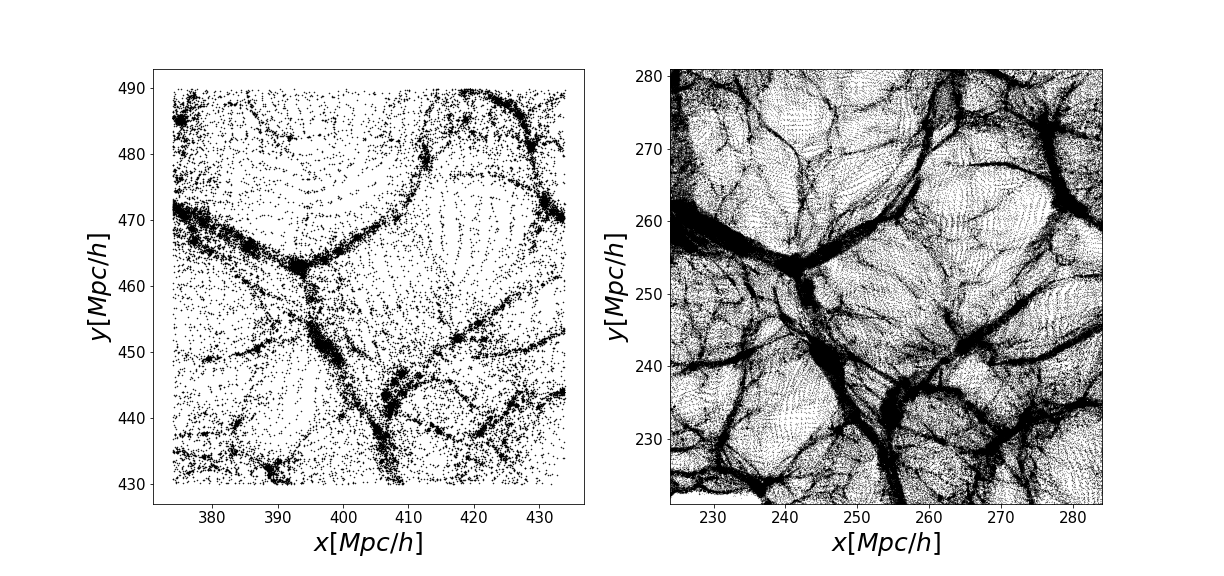
\includegraphics[width=15cm]{Figures/Resi.png}
    \caption{Caption}
    \label{fig:my_label}
\end{figure}{}


En la figura \ref{VoidsIn} se presenta el gas contenido en ambos voids. Ambas secciones pasan por el centro de los voids y la seccion transversal se corresponden al diametro de los voids proyectados sobre el eje z. Los gr\'aficos fueron realizados con el c\'odigo publico \texttt{\textbf{SPH-VIEWER}} \citep{SphViewer}. Este c\'odigo permite estimar los campos de densidad a partir de la implementaci\'on de la t\'ecnica de SPH introduciendo las \textit{longitudes de suavizado} de las particulas. \textbf{PONER ALGO DE ESTO EN LA PARTE SPH CAPITULO}.
\begin{figure}
    \centering
    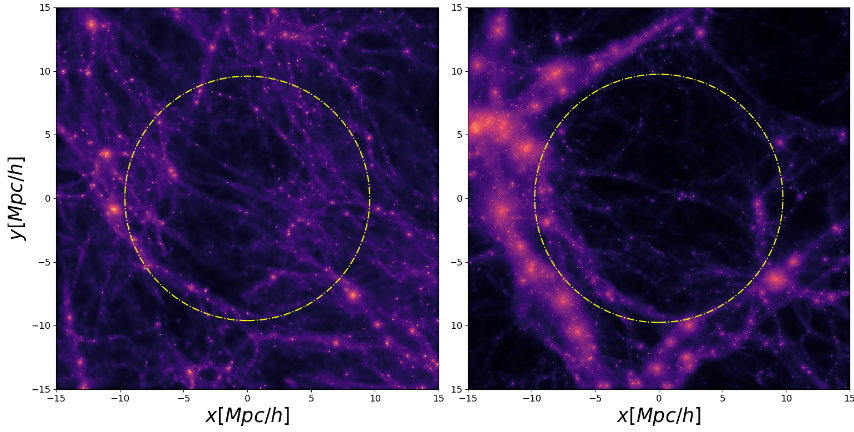
\includegraphics[width=15cm]{Figures/SphVoids.png}
    \caption{Caption}
    \label{VoidsIn}
\end{figure}{}
A partir de \ref{VoidsIn} puede apreciarse como las resimulaciones permiten la obtenci\'on de subestructura dentro de los voids. Podemos ver como estos estan atravezados por una fina red de filamentos y ciertos halos. En el caso del void R, vemos como este carece de una pared sobredensa a diferencia de el void S (derecha) donde vemos como esta envuelto por una gran sobredensidad con importantes nodos. 


\section{Perfiles}




\begin{figure}
    \centering
    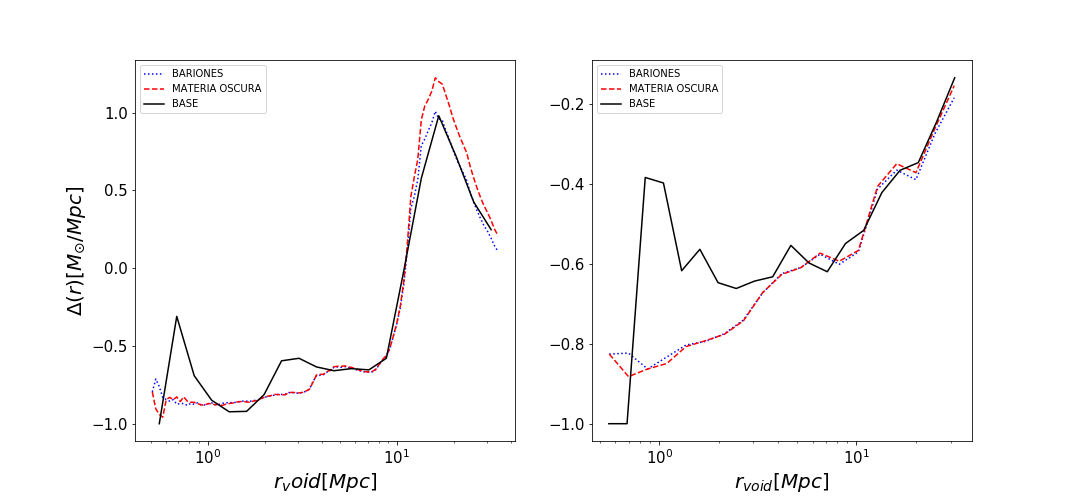
\includegraphics[width=\linewidth]{Figures/PerfilesIntegradsos.png}
    \caption{Caption}
    \label{fig:my_label}
\end{figure}{}

\begin{figure}
    \centering
    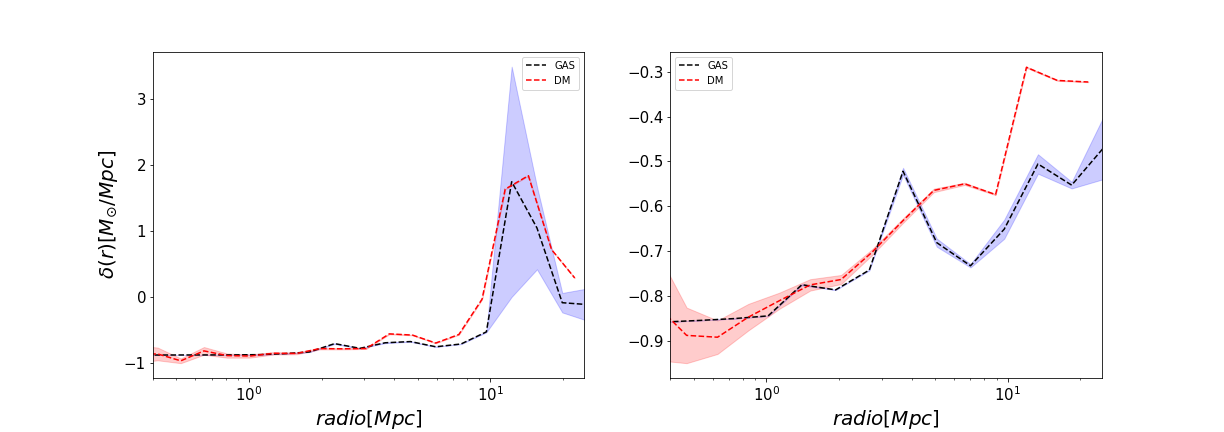
\includegraphics[width=\linewidth]{Figures/perfiles_sph.png}
    \caption{Caption}
    \label{fig:my_label}
\end{figure}{}